% !TeX root = ../AnalyticStacks.tex

\section{\ufs Berkovich spaces (Clausen)}

\url{https://www.youtube.com/watch?v=fnEPiDIF9_k&list=PLx5f8IelFRgGmu6gmL-Kf_Rl_6Mm7juZO}
\renewcommand{\yt}[2]{\href{https://www.youtube.com/watch?v=fnEPiDIF9_k&list=PLx5f8IelFRgGmu6gmL-Kf_Rl_6Mm7juZO&t=#1}{#2}}
\vspace{1em}

At the very beginning, in the first lecture, I gave an introduction to what we wanted to have out of this theory of analytic stacks.

% 0:43
In particular, I was putting some emphasis on the fact that we want to know that traditional frameworks for analytic geometry can fit into this perspective of analytic stacks.
% 0:53
We have already discussed adic spaces and a little bit of geometry over this, like Tate curves. 

\textbf{Question:} With adic spaces, there was this issue of shifting and then the idea was that you have to define some kind of derived adic spaces. This will not explain in full what is Huber \note{something I didn't hear, derived ... spaces}. This will not fully explain what is derived Huber \note{I could not hear this part} set up and in your formul. 
% 1:23
Maybe there are different ways to do it. I'm not sure.

\textbf{Answer:} It's possible there are different ways to do it. 

\textbf{Question:} This is already in progress?

\textbf{Answer:} Let's say that. 

% 1:32 Peter

It's in Juan Estaban's paper on the analytic de Rham stack Camargo \cite{AnalyticRhamStackRigid} \note{Not sure if I should cite with the name Camargo or Estaban}. So, there you go. 

% 1:55
What I want to start moving towards today, is the relation with Berkovich spaces.

% 2:10
But before discussing that, I want to do a little bit of setup. First, I want to talk about \emph{different notions of how to localize an analytic stack over a topological space}. 

\subsection{Localizing an analytic stack over a topological space}
% 2:40
We have already seen one way. 

If we have an analytic stack, and if we have an $S$, which is a metrizable, finite dimensional, compact Hausdorff space, or it could be a locally compact Hausdorff space, which is locally one of these, then we've seen that this can also be viewed as an analytic stack. Then we could ask for a map $f: X \to S$ in the category of $\AnStack$. 
% 3:25
We discussed what structure you get on $X$. Basically, you get a bunch of idempotent algebras in $D(X)$, corresponding to the closed subsets of $S$. You can also think in terms of the complementary opens as well, and you get some idempotent coalgebras which would be like the $D_{!}$ \note{Not sure if D or J} of the constant sheaf on the open subset, as opposed to the $I_{*}$ of the constant sheaves, giving you these idempotent algebras. But, in any case, you get a whole bunch of algebra objects in here $D(x)$, which let you localize this category over the topological space $S$.
% 4:05
But when discussing the relation with Berkovich spaces, it's going to be too annoying to require these kinds of conditions (metrizable, finite dimensional, compact Hausdorff), even though they're satisfied in practice. So, I want to discuss some slightly more general notion of how to localize an analytic stack along a topological space and the relation with this one in the case where you do have a metrizable, finite dimensional, compact Hausdorff space.



So what is another thing I can do? If you have an analytic stack $X \in \AnStack$.
To $X$ we can assign a locale. We call it $\Loc(X)$, which is given by the monomorphisms in analytic stacks.

\[
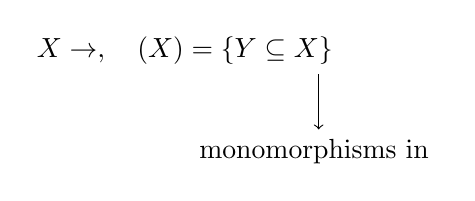
\begin{tikzpicture}[baseline=(current bounding box.center)]
    \node (A) at (0,0) {$X \to \Loc, \quad \Loc(X) = \{ Y \subseteq X \}$};
    \draw[->] (1.7,-0.3) -- (1.7,-1.0);
    \node[below] at (1.7,-1.0) {monomorphisms in $\AnStack$};
\end{tikzpicture}
\]


% 5:03
So this is a general thing you can do whenever you have a topos, or an $\infty$-topos.
It always has an underlying locale, where you only look at the monomorphisms. And if you look at the topos axioms, then you can see that unions...

\textbf{Question:} Here that possible infinite unions and intersections exist? \note{I did not hear this well}

% 5:32
\textbf{Answer:} Yes. But, I should say that potentially there are some set theoretical difficultie,s so that potentially $Loc(X)$ is not a set. I did not investigate it seriously. But in a few seconds, you will see that it doesn't matter, when I get to the definition.

\textbf{Question:} Do you mean, when you get larger and larger sizes, you could have more and more subobjects.

% 5:48
\textbf{Answer:} In principle. I didn't spend much time to prove that it is a set, because ...


\textbf{Question:} About the locale axiom, you said there is a way to produce finite binary intersection and unions, but you also have to produce infinite, I mean...

% 6:12
\textbf{Answer:} This category $\AnStack$ has all limits and colimits. We don't have to do anything special here to make this definition work.

% 6:20
\textbf{Question:} Why is the colmit a submonomorphism? Ah, you take the colimit and then you quotient by the... \note{I did not hear this well}

\textbf{Answer:} That is a general $\infty$-topos thing, for example you could take the Cech-nerve of the map and take the colimit.


\textbf{Question:} And this is in what kind of $\infty$-topos, the analytic stack?

% 6:49
\textbf{Answer:} Yes. Modulo set theoretic technicalities. So it satisfies all the same exactness as an $\infty$-topos, but it is not presentable, so...

% 7:00
\textbf{Question:}  OK, so it could be some...

% 7:10
\textbf{Answer:} So maybe $\{ Y \subseteq X \}$ is not a set, I don't care, and you'll see when I make the definition.

% 7:12
When I make the definition that I'm interested in, it doesn't matter whether it's a set or not. 

\textbf{Question:} The monomorphism, if I only consider \note{I did not hear this} that's like taking connecting component. 

\textbf{Answer:} Exactly, so it means that if you do the fiber product of  $\{ Y \subseteq X \}$, then the diagonal, I mean the diagonal map associated to this inclusion is an isomorphism.

\begin{unfinished}{7:40}
% 7:40
A topological space also gives rise to a locale. But let me actually change perspectives and just say "$S$ is a locale", instead of saying "$S$ is a topological space". 
% 7:52
Then we can ask for a map of locales, $Loc(X) \to S$. Whether or not $\{ Y \subseteq X \} $ is a set, this is some data that makes honest mathematical sense. A locale is by definition the collection of open subsets, which is a set. You are saying that for every open subset, you have to give such a monomorphism, and  unions have to go to unions and finite intersections have to go to finite intersections.

% 8:26
\textbf{Question:} In the literature about locales, I don't remember, I don't use it much, but this is like the direction of map of topoi \citeme{}, but I don't know when they define M of locales \note{I did not hear this}, is it in the other direction or in this? 

\textbf{Answer:} I don't know either. So I'm doing the geometric morphism, let's say a geometric morphism of locales. 

\textbf{Question:} Well, morphism of sites...
\textbf{Answer:} Morphism of sites goes the other direction. I'm talking about a geometric morphism. 
\textbf{Question:} But also a morphism of sites \note{I did not hear this}

but also of goes in the direction.

\textbf{Question:} For locales it is not used much by algebraic geometers.

% Back to lecture
% 9:26

But we can also ask for a stronger property, so that each inclusion of open subsets, say $V$ inside $S$, maps to, so it's supposed to give some monomorphisms, so maybe I should give some name for this, like $f$ or $Pi$, maybe. So this goes to $\pi^{-1} U \subset \pi^{-1} V \subset X$. We could ask that these inclusion maps are actually open immersions from the perspective of the six functor formalism that Peter discussed last time. That is, the extended six functor formalism on analytic stacks. So we could ask that each of these inclusions be shriekable, and that they be well cohomologically smooth.

But in the case of a monomorphism, then it's quite easy to see that the dualizing object is canonically the unit, and it's the same thing as an open immersion. A general monomorphism could look like anything really, it could look closed, it could look open, it could look like some mix. But it's reasonable to ask for this stronger property, that what looks like an open immersion on the level of the topological space also looks like an open immersion from the perspective of the six functor formalism.

% 11:24
In the case where $X$ is a metrizable, finite dimensional, compact Hausdorff space, we can ask for, as before, a map $X \to S$ in $\AnStack$.

% 12:00
\textbf{Question:} When you say $S$ is a locale, what is the definition of a locale? What does it mean for $U$ to $V$ an open set \note{I did not hear this}?
\textbf{Answer:} I'm using a bit of loose terminology here. But the definition of a locale is that it is a certain poset. That axioms that you impose on this poset are the axioms that are satisfied by the poset of open subsets of a given topolocal space.
% 12:30
But by abuse of notation, I'm using this symbol $U \subseteq S$ to mean that $U$ is an element of the poset which $S$ is secretly. But it is because I am thinking of it as a topological ... \note{I didn't hear the last word}


\textbf{Question:} Equivalently \note{todo}

% 12:53
There is another perspective, it goes like this. You take the definition of a topos but instead of sheaves of sets you look at sheaves of truth values. I don't know if this is helpful or not.

%13:08
An usual topos would be a $1$-topos. Then a locale maybe would be a $0$-topos or something like that, I don't know.

%13:25
If you have this kind of structure, then you get \note{todo}
Note also that if you fix $X$ in $S$ ($Loc(X) \to S$ \note{$\pi$ above arrow}, \note{todo} they are all just sets. They are not anima or whatever, because here we just asking for a map of locales. It is just a map of posets in the other direction. 

\textbf{Question:} Not that when you say set, it also means in this sense of the set theoretical size difficulties.

% 13:56
\textbf{Answer:} That's true. So, up to size difficulties. I mean, there are no automorphisms of any fixed on of these $$Loc(X) \to S$. There are no non-trivial automorphisms. That is a good point. 
% 14:11
So this is tautological. Why does this imply this \note{add what is being pointed at}? Basically, you can just check on the level of the analytic stack associated to such a guy that every open inclusion, actually is an open inclusion from the perspective of the six functor formalism. Peter more or less discussed this last time, that our six functor formalism on analytic stacks, when we restricted to this case, recovers the usual six functor formalism on locally compact Hausdorff spaces. And then this property of being an open immersion is stable under base change

% 14:54
\textbf{Question:} So can you say so you know that open immersion holds for, ah, it is stable under, of analytic stacks or \note{I did not hear this}

\textbf{Answer:} It's stable under pullback.

% 15:16
This is the strongest condition. If you have this, you can ask whether this holds \note{add what is being pointed at}. You check whether certain inclusions or open immersions, if you have this, you can ask whether this holds. As we discussed the last couple of times, that corresponds to some connectivity condition on the idempotent algebra, as you see. 


% 15:36 Example is started, but there is a question. The example is restarted at 17m10
The second one is given off by, lo, is one of open, opener, that's true. You could think of this in terms of there's, lo, local X, and then there's some quotient local which is like the local of monomorphisms that are open versions with respect to the six functor formalism, and then the second bit of data is a map like this, thanks for that remark, Peter.

And is it the case that the union, maybe I go confus, union of open immersions is an open immersion or to make it an open, no, that's true, that it's an open immersion, which is needed to, well, it's needed to, it's needed to have this local, I mean, so, or well, remote, I mean, depends on how your, whe. No, but it's true, so that if you have a union of open immersions, then it's still an open immersion, and that's an important point to check when you're discussing these things, and it follows from this extension procedure for six functor formalisms that Peter discussed.
% 17:06
If you have a union along open immersions, then those are sheafable maps, and but it's also a cover, and you can get a a lower shriek map defined on the union and then you can actually check locally that it's cohomologically smooth.


% 17:10
\begin{example}[\yt{17m48s}{Huber pair todo}]

Let's give an example. Remember way back when we had Huber pairs $R, R^{+}$ and stuff like that. Then we assign to this an analytic ring $(R, R^{+})^s$ \note{todo} solid. Then, we can take its spectrum, and then we can look at the locale $Loc(Spec)$ associated to this. What we essentially already saw, was that this analytic stack localizes along the usual Huber topological space of continuous valuations $\Spa(R, R^{+})$.
\end{example}

% 18:14
\textbf{Question:} Now you consider the spec in your, \note{todo}


\textbf{Answer:} This is what this is, spec n. So, I'm lazy, I say $\Spec$ 

\textbf{Question:} And then, $\Spa$ in the old sense.
\textbf{Answer:} Yes. 
\textbf{Question:} It's a topological space
\textbf{Answer:} Yes. 
\textbf{Question:} And then, okay, the local, okay, and then you have a map of, oh, 

This loc, this means for every open in the add space, you give a monomorphism of analytic stacks. Of course, this involves passing to some derived Huber pairs in some sense.
\textbf{Answer:} Yes. 
\textbf{Question:} Because you are not, but your original pair is is not derived. 
\textbf{Answer:} So on the level of rational opens, this is going to give another affine analytic stack, which is the one where you enforce that $F$ invertible. In the world of analytic ings, you enforce that $F$ is invertible, and that $\frac{G_1}{F}, etc., $\frac{G_N}{F} is solid.
% 19:45
That defines some analytic ring. under this analytic ring here, and passing to $\Spec$ it is a actually a monomorphism, on the level of the derived categories for example it is a localization. 
% 20:04
That gives some inclusion of analytic stacks here. What we argued 
% 20:15
We proved a less precise version of this claim early on, when we argued that the derived category 

% 20:30
So this refines the statement that $D(R, R^{+}) solid$ \note{todo}$ localizes on $\Spa(R, R^{+})$.
% 20:48
Recall that you have a sheaf of $\infty$-categories on this topological space $\Spa(R, R^{+})$, whose global sections is equal to this $D(R, R^{+}) solid$, and whose sections on a rational open is the analogous category where you impose these conditions \note{todo, add latex}/

% 21:00
We had several discussions about when this is the same as \note{todo}

Can always refine any open cover here so that, so in fact, you get an open cover. So in fact, we showed, without having the L, without having introduced the language for it, we showed that any open cover or cover of a rational open in $\R^+$ pulls back to an open cover, can be refined to, pulls back to an open cover of, you know, the, pulls back under $\Pi$ to an open cover in the sense of the six functor formalism.

\begin{remark}
Let me make an open cover to cover by monomorphisms. In general, it's not true that a rational open pulls back to an open immersion. 
\end{remark}


\begin{example}[\yt{23m44s}{Remark example, todo}]
Is there a proof of this? I'll give an example right now.

% todo, correction in lecture
So, have two formal variables, $p$ and $X$. Oh, sorry, I should say $\Z_p$. I don't need two variables. Thanks. So one formal variable and then invert it. 

$ (\Z_p, \Z_p) \to (\Q_p, \Z_p)$
What does this correspond to? On the level of analytic rings, we get this, and on the level of derived categories, this is solid $\Z_p$ modules, and then this is a, well, this is algebraically inverting $p$. The left adjoint here is the inclusion of the full subcategory, or the right adjoint here is the inclusion of the full subcategory where $p$ is invertible.

So this passing from $\Z_p$ to $\Q_p$ is algebraically inverting $p$, $p$ is a prime. And that actually, from the perspective of the six functor formalism, is a closed immersion, not an open immersion. That's a proper map because the, this hasn't the second variable hasn't changed, so we're changing the underlying ring and not the analytic ring structure. But it's also a, proper monomorphism, it's a, it's a closed inclusion, it's closed, not immersion, not open.

So, I think we treated the case of some covering given by a function like $f$, like the Laurent cover, the one where $f$ or $1-f$ is less than or equal to mean, this kind of basic cover. And for those, is it the case? Yes, so then let me make another remark. However, if $R$ is Tate, then indeed, this doesn't arise. So in general, the problem is exactly these open covers in the Huber sense, which are given by algebraically inverting a function without enforcing any inequalities. But in the setting of a Tate Huber pair, then you know, if you want to invert something, it's, the subset where you invert something can always be written as a union of subsets obtained by forcing inequalities.

So, it is not quasi-compact in general, right? But dealing with something which is in the sense of the ADC space is quasi-compact because it is a rational domain. I think in the, yes, but I mean, it is Rush, so it is quasi-compact in the, yes, in the. This also has to do with the fact that we didn't directly, I was sliding one little thing under the rug here, which is we didn't really directly define this as a map. We didn't really directly define it like this, remember we actually had this valuative spectrum of all of these guys, and we actually defined this map and then we used Huber's retraction here. So this was not quite accurate, because that would be accurate on the level of $\Spa$, but that's not exactly how we get it for $\mathrm{Spa}_a$. Instead, we, assume that the real $\mathrm{Spa}_a$. The idea is open, and then it's okay.

So, the point is that the rational opens in the Tate case can always be described by forcing inequality among the valuations. Okay, let me try to finish what I was trying to say. I want to give an idea of what's going on, I don't want to get too precise about it, but it's this kind of phenomenon, where these guys correspond to this kind of thing, which does correspond to an

So, sheets on this $F$ is not there. In fact, you cannot algebraically invert $F$, but using the right-hand side. That's right.

Okay, and also, there is another topology on the same space, with the same constructible subsets. Where the open pulls back to open.

So, another fix, even outside the Tate case, is to choose a slightly different topology from the one Huber described, where both of these things are open. It's not the constructible topology, no. It's a topology which is incomparable to the Huber topology. For this subset here, $P \neq 0$, it will be closed from one perspective and open from the other perspective. It's open from Huber's perspective but will be closed from the perspective of this other topology.

It is a spectral space. To be open, you basically redeclare Zariski open subsets to be closed, which the Zariski open they are not.

For example, inverting $P$ here, inverting $P$, is now closed in the new topology. We haven't discussed that element of synthetics so far, that's true. But let's leave that aside, I think there's already enough information being discussed.

Is it the opposite spectral space? No, it's not the opposite spectral space, because these ones are still the ones where you're enforcing inequalities like $f \leq 1$, that's still open in both cases. It is the opposite of one of the ones Huber describes in one of his papers.

Yes, we can make this more precise. I'm going to hesitantly say yes, it's obvious if you remember the definitions of everything. Maybe we need compact or not, because I mean, you want an input to correspond to it, but I'm not sure whether if it's not quasicompact, you have...

So everything is defined by inequalities $f_i \leq g_n, g_n \neq 0$, and this one you replace by saying that is a closed condition for any $G$. Well, I mean, you have a rational open, so the conditions are satisfied, like the ideal generated by all of them is open. So, you can't invert $G$ if that doesn't correspond to a rational open in Huber's sense, but in situations where you can, it corresponds to a closed conclusion.

One last remark about this general setup: if $S_i$ is some inverse system of compact Hausdorff spaces, then giving compatible maps from $\operatorname{Lal} X$ to $S_i$ for all $i$ is equivalent to giving a map from $\operatorname{Lal} X$ to the inverse limit. And it's the same for $\operatorname{Lo}_p$. If all of those ones factor through $\operatorname{Lo}_p$, then this one will also factor through $\operatorname{Lo}_p$.

Every compact Hausdorff space is a limit of metrizable finite-dimensional spaces, potentially in many different ways, but in many situations, there's a natural way of doing it. We'll see this in the setting of adic spaces, and then this gives you a way of going from the case of metrizable finite-dimensional compact Hausdorff spaces where you can sometimes go from this perspective and you can go to this perspective.
You're closed, you know, the situation kind of passes to inverse limits in a nice way, but now you no longer have to worry about things being metrizable or finite-dimensional. Okay, that was my little, is a map to s the same thing as a map from loal? No, because you have this connectivity condition, so it's the you still have to impose this locally that locally all the item poent algebras are connective. I mean, as far as I, it's not like I produced a counter example, but I kind of believe that it's not the same.

Okay, so I'm always confused, is there really a t-structure def over D of that object? And no, no, there's no t-structure. So what I didn't, I don't have to say what I mean by connective. I have to say what I mean by connective locally, and what I mean by connective locally is that there exists a cover by apine things such that it's your object when you pull back to each of those apine things is connective. Now, once you're in the apine world, connectivity is a pullback of something connective, is you have a t-structure and the pullback of something connective is connective, so it's kind of. And also, if the pullback is connective, then it's connective or not, no, that that is not necessarily true, okay, okay.

Okay, so it's not like, so it's not a sufficient condition for having a. So this is like the for schemes that you have the the non-aine orens, but still, if you use as the flat or pqc, still if it's up upstairs, it's up downstairs, so that's. But in your topology, of course, you have much more stuff, yes. So you can have these wheel-we things where, you have a map which is affine locally, but with an with a map with affine Target which is affine locally, but not globally, and that's kind of unavoidable when you're doing analytic geometry.

% 40:05
\subsection{Preliminary definitions}
\subsubsection{Banach rings}
So Berkovich spaces. Let me start with a reminder on the definition, so we know where we're going. $A, \norm{\cdot})$ is a Banach ring. That means that $A$ is a commutative ring, and this norm map $||: A \to \Rnonneg$ from $A$ to the non-negative real numbers ,satisfies, 

$\norm{0} = 0$, 
triangle inequality, $\norm{x + y} \leqslant \norm{x} + \norm{y}$ , 
and third of all, it's sub-multiplicative.
$\norm{xy} \leqslant \norm{x} \norm{y}$
So, probably have to put the norm of -1 is equal to the norm of one, which is e z, I should probably put that, so either a equal Z or Norm of 1 equal 1 and Norm of us one, also do you need that? It does not follow I'm not sure how much it follows, but it, it's usually they want the triangle inequality Al with x + y, okay. I think you can, you can get it, you can give a crazy thing like the negative multiply by two, you can do something that still satisfy the a without, but of course, it would be equivalent something satisfying the a, this is probably not how to show, okay.

Then $A$ is complete, with respect to the metric $d(x,y) = \norm{x-y}$. 

\begin{example}[\yt{42m24s}{Banach ring}]
So an example, there's, so example for, say, $S$ is a compact hausdorff space, you could take for $A$ to be, say, complex-valued continuous functions,
$A = \Cont(S; \C)$

 and take the norm to be the sup norm, where you have the usual absolute value, and this, maybe this is kind of right. 
$\norm{f} = \sup_{s \in S} \norm{f(s)}

\note{todo, last bit of eq I can't see}
\end
 
\begin{example}[\yt{43m04s}{Tate-Huber ring}] 
 Another example would be if $R$ is a Tate-Huber ring, and if you choose a pseudo uniformizer, topologically nilpotent unit, then you can define a norm, Peter actually wrote down the
\end{example}

Yes, this is multiplicative. It's not multiplicative in general.

\begin{align*}
(A, \norm{\cdot}) \leadsto \BerkSpec(A, \norm{\cdot}) = \{ \norm_{x} = A \to R todo \} \\
\text{\underline{multiplicative seminorm}} \\
with \norm{f}_x todo \norm{f} \\
\forall f \in A.
\end{align*}
And then so to this data, so this to a and the Norm Huber assigned the space, which has a set Berkovich. Thank you, we're switching over now. Thought Berkovich, which as a set is given by the. Norm of $f$ equals $z$ if and only if $f$ equals $z$, right.
% 46:30
So, I'm using this notation $X$, so kind of it's a decoration to. And this is now a \underline{multiplicative seminorm}, with which is bounded by the given norm you have on the Banach algebra $A$.

\begin{example}[\yt{47m13s}{Tate-Huber ring}] 
\begin{align*}
A = \Cont(S, \C) \\
\norm{f}_x = \norm{f(x)} \forall x \in S.
\end{align*}
Well, for example, in and you can take. If you require that the norm restricts to the usual Norm on the complex numbers, then these are all the examples. So that's  Gelfand's theorem. So, those are the only examples in this situation. And multiplicative includes the of Zero element, that is the norm of one is one, yes.

Except, but this is maybe zero multiplication of zero numbers, we don't want that. So, we want these to be like points, so we want them to be non-empty. So, we want one to be different from zero.

But, do you allow $\Z_R$? No, well, wait, I allow, okay, I allow $\mathbb{A}$ is the zero ring, when this will be the empty set.

\begin{align}
\BerkSpec(A, \norm{\cdot}) \subseteq \prod_{f \in A} [0, \norm{f} ]
\end{align}
This is actually a compact Hausdorff space. I didn't describe the topology, but here it is. You can view it as a subset of the product over all $F$ in $A$ of the interval from zero to the norm of $F$. It is actually a closed subset. This map takes a norm and records its value on $F$. The topology is the subspace topology, so it is a compact Hausdorff space.

\subsection{Berkovich spaces in the language of analytic stacks}
% 50:20
So what we're going to do is, we're going to try to make the same definition, but in the world of analytic stacks instead of topological spaces. So, we want to take the same idea, which is that we want to look at the set of all multiplicative seminorms $\BerkSpec$ on $A$, bounded by the given norm on $A$, but we want to say that in the language of analytic stacks, using the notion of norm on an analytic ring that we discussed earlier.

% 51:18
Let me remind you about this notion of a norm. So, the definition of, well, we could say even more generally in an $\infty$-category stack. 

% TODO: when the earlier lectures are transcribed, we can see what we need to copy here.

A norm on $X$ is a map from the algebraic $\P^1_X$ to the closed interval from zero to Infinity, including Infinity, which is multiplicative away from Infinity. So, let's say on Norm inverse $0$ to Infinity, and let me write it suggestively like this. You really should write down the commutative diagram with inversion on $\P^1$, inversion of the coordinate on $\P^1$ and inversion of this extended real positive non-negative real axis here. And some condition on how $\mathcal{P}$ sits, $p$, $p$, $p$, so this is the $p$, oh $t$, $t$ is the variable on $\P^1$.

Yes, what do you mean by how $\mathcal{P}$ sits? So, remember $\mathcal{P}$ was this ring object you have over any analytic ring, which is the free guy on a topologically nilpotent element. And it's some version of a unit disc, and what we ask is that this Norm function gives

Small $a$ map in the category of analytic stacks. So these objects are fixed, right? When you fix $X$, this is fixed, and this is fixed. Yes, that you know that there is a. Why was it? Well, we basically by definition, every analytic stack was a small co-limit of representable analytic stacks, okay? You have a.

Because there was a notion of analytic ring where there is the category. Okay, there, you handle the problem of large sizes. I mean, because it's enough to check the condition some smoke, but then you have the analytic stack where you cover, but you don't know which covering you need to give a ism, so you have need all possible covers could be covers by bigger and bigger see, but you say the category is accessible. So the main technical result you need to prove is that the sheafification of an accessible prief is still an accessible prief. That's the main technical result you need to prove. We did not discuss this at all, but that's what's underlying the resolution to these issues. It's like in Waterhouse.

Okay, so this, in fact, so there's a cover, so this gaseous base maps to $n$. In other words, you can write down a norm on this gous space tack, and it's, and this, so this, and this is actually the universal norm on an analytic ring with a variable $Q$ in $R$ such that norm of $Q$ is precisely equal to $1/12$. What did you write? $NX$ is the analytic stack $n$, $n$ is an analytic stack. So $NX$, the set of norms, is actually the set of maps from $X$ to some stack $n$.

So if you ask for a norm on an analytic ring and an element whose norm is exactly equal to $1/2$, which is kind of a somewhat stringent condition, because a priori again, the norm map is norm of $Q$ is a map from $Spec R$ to $[0, \infty)$, and you're asking that it factor through this, a priori, its image could be some interval or something, but you're asking that its image be exactly this singleton. The universal example of that is this guy, and moreover, the map to the base stack is actually a cover in the sense of our Gro de topology on analytic Stacks, because every norm on an analytic ring locally, you can find such an element. We had this argument, we discussed this two lectures ago. Everything here was like $X$ was a $Spec$ of an analytic rate. I mean, I made this definition for a general $X$, but it, I mean, it doesn't matter because the condition, I mean, the norms on an analytic ring, they satisfy descent basically. I mean, it's kind of follows from general nonsense, and so it automatically glues to say what a norm is on an arbitrary analytic stack, and it unwinds to the same thing. So the cover also exists because it exists locally, like you GRE it. Well, the map, the map, no, the map exists because you can write down this norm, and then it's a cover because given any norm on an analytic ring, after a cover, you can find a $q$ that satisfies this property.

Sure, do you need to do some base tank? I'm sorry, do you need to do a base change? What do you mean? Is it okay, or you still have a question?

Okay, so I want to, before finishing the discussion of or introducing the definition of this enhanced Berkovich Spectrum as an analytic stack, I want to explore a little bit about so, what does $n$ look like? So, well, what do we have on $N$ if you have a norm on an arbitrary analytic ring? So, if you have a norm $p: R \to [0, \infty)$, so as mentioned, for any section here, you get a function from $Spec R$ to $[0, \infty)$, but over an arbitrary analytic ring, the only thing we know exist are the integers. So, given $n$ in $\Z$, we get a map which records the value of your norm on the integer $n$. So, what does this
We'll also see that the fiber over any point in the image is non-empty, so that at least in this case, maybe it's a general fact - I don't know, at least in this case, it's kind of a theorem that the image is closed, so to speak. Now note that the more traditional thing is this Berkovich spectrum of the integers, that was also by definition a subset of this product going from zero to infinity, and it was given by those Norms, so multiplicative, avoiding Infinity, satisfying the triangle inequality.

Let me remind you what this thing looks like, in case people haven't seen this before. Recall that $\M(\Z)$ looks as follows: you have a point at the center, so to speak, which corresponds to the trivial norm, meaning the zero norm of $Z$ is $Z Norm$, and the norm of everything else is equal to one. 
% 1:05:33
Then, you have several branches. You have an archimedian branch, so at the end of the archimedian branch, you have the usual norm, the usual archimedian norm, the usual absolute value. But then, for each prime $p$, you have another branch, which also ends at some point. To get the correct topology on embedding it into $\R^2$, you should probably make the branches get shorter and shorter and shorter, but okay, that's...
% 1:06:10
But the situation with these $p$-adic branches is a little bit different. So, what's going on here? Here, you have the usual absolute value, and here, at the halfway point, you have the square root of the usual absolute value. And here, you can then you can put any $\alpha$ between zero and one, and you can kind of see from the intuitive perspective that this interpolates between the usual absolute value and the trivial absolute value. 
% 1:06:34
Here, what goes at the top is not the usual $p$-adic absolute value; the usual $p$-adic absolute value sits somewhere here, so normalized to say so that P equals 1 over p. And now, you can actually scale it to $R_{>0}$, and then there's also a limit as the scaling goes to infinity, and what that gives is the trivial norm or the pullback of the trivial norm on the residue field $FP$, so in other words, the norm of any multiple of $p$ is equal to zero, and the norm of everything else is one.

Okay, what of course, no, I... This is great. I think this was something like this, this is the first talk. There was a talk in this course, it was in this course or another, probably in this course, there was some discussion of, but maybe I could do this another thing. 
% 1:07:42
So I'm trying to recall something which is well-known indeed, in order to set up the discussion of what's following here. So, in particular, I want to emphasize this is a really big space, but the subspace $MZ$ \note{todo} is quite small, you know, one-dimensional.

\textbf{Question:} So, now what we're going to see, so there, you allow the value to be in, but here, you don't. 

% 1:08:13
\textbf{Answer:} That's correct. So, here's going to be the claim: the image of the norm $\text{Im}(\mathcal{N})$ is a larger subset. It looks like this: you have all the same ones as before, sorry, I'm trying to say that it stops there, trying to draw like a closed interval sign, but then also at the archimedian place, it gets extended. So, here now the usual archimedian absolute value is also in the middle of the interval, and you can take arbitrary powers of it, so for any $\alpha \in R_{>0}$, you can take powers of it. So, it'll go to there in one direction, and to the other direction, you get some really strange point, which corresponds to... 
% 1:09:23
So, it's a subset of there, so it's given by some maps from $\Z$ to the extended real line there, and it's given by $N(n) = \infty$ if $n \neq -1, 0, 1$.

% 1:10:17
\textbf{Question:} \note{todo}
\textbf{Answer:} No, it is a different kind of base. Because over Solid $\Z$, $\R = 0$ you can't.

\textbf{Question:} \note{todo}
% 1:11:18
\textbf{Answer:} It extends to to infinity and then compactified at the end. You can try to write a formula for it. It's like the image norm is like - you take the Berkovich space of the integers. Ah, no, let me make a before I say this.

% 1:11:35
In particular, the triangle inequality can fail. That's quite clear here - you have $N(1) = 1$, but $N(2) = \infty$. That's a pretty drastic failure of the triangle inequality. But also, like for the square of the usual absolute value, which is a new thing, you have the triangle inequality fails as well.

% 1:12:05
So, another way of saying this is $\text{Im}(\mathcal(N)) = \BerkSpec(\Z)$ - you can get it from the Berkovich spectrum of $\Z$. On the Berkovich spectrum of $\Z$, you have an action of the real numbers greater than or equal to one. Wait, did I - or well. Or maybe, on this other thing, you have an action of the positive real numbers. You can do this, and that doesn't do anything on the non-Archimedean branches, and then on the Archimedean branch, it extends it all the way, and then you compactify it - one-point compactification. So, I don't know.

Let's explore this and let's see what is going on. Let's consider the map - what's that? Is the one-point.

\textbf{Question:} The picture you seem to see this image gen topological space, but this is supposed to be something associated with $\Z$, right? That's a good question. So, by definition, I made it a - I was saying it's a closed subset of the topological space. Now, you can view this as an analytic stack. We saw how to view this as an analytic stack, and you can take the product in the category of analytic stacks - that's perfectly legitimate. It's no longer finite dimensional - sorry, it is metrizable, it's no longer finite dimensional. So, we didn't quite talk about this thing, but you can still view this as an analytic stack, and you still do get a map of analytic stacks from N to this product, and this closed subset does correspond to a subanalytic monomorphism of analytic stacks here, and the map from N there does factor through that closed subset, and so you can view it in several different ways.

% 1:13:00
Okay, to explore this, consider a fixed prime $p$, and consider the norm of $p$ 
$
\mathcal{N} \xrightarrow{N(p)} [0, +\infty]
$
. 
% 1:15:15
Here's the first claim: we can understand the locus in this universal space of norms where the norm of $p$ lives in [0, +\infty]. This is the same thing as the stack parametrizing norms on which the variable $p$ lives between 0 and 1 - let's call this $N$ and $\Z$ less than absolute value of p less than one. This is equal to $\Spec \Q_p^{\gas}$, the gaseous version of the $p$-adic numbers, across this stack associated to the open interval $(0, 1)$.

Claim
$
N(p)^-1 ((0,1)) = $\Spec \Q_p^{\gas} \times (0,1)$ 
$
% vertical equal sign
$
\mathcal{N}_{0 < \abs{p} <1}
$

This is quite easy to see, because we know that the universal analytic stack equipped with some variable whose norm is between zero and one \mathcal{N}_{0 < \abs{p} <1} is spec of $\Z_q$ hat plus or minus one Gaseous cross 0,1. And then you have to impose that that variable becomes p, so you set $q = p$ or you mod out by $q - p$, and then that, as Peter discussed when discussing this gaseous base stack, gives you some analytic ring structure on the $p$-adic numbers, and then the second variable doesn't really change.

% 1:17:40
I'm claiming in particular that if you look at the universal - let's say we take the fiber over a point $ \lambda \in (0,1)$, 


$
Spec(Q_p^\gas) \times \{ \lambda \}      \text{normed analytic ring structure \\ here: notion of overconvergent functions on a disc of radius $r$ }
$
then you get a normed analytic ring structure here. And it is - so what does that mean? It means that for every radius $r$, you have some notion of overconvergent functions on a disc of radius $r$, where the notion of on a disc of radius $r$ is the usual one from non-Archimedean geometry, where you take the normalization of the absolute value on the $p$-adic numbers for which $\abs{p} = \lambda$. So, what we're seeing here is the interior of the $p$-branch.
Kind of fairly straightforward to understand. 

% 1:19:54
Next, let's look at another locus that's fairly easy to understand. This is the locus where $p$ is between one and infinity. 
\begin{align*}
\mathcal{N}_{1 < \abs{p} < \infty} = $\Spec(\R^\gas) \times [0,1]$

% todo arrow between above and under

0 < \abs{\frac{1}{p}} < 1

\end{align*}
% 1:20:10
Strictly between one and infinity, because that's the same thing as saying that $p$ has to be invertible. The absolute value of $p$ is away from zero. 
% 1:20:20
Then it's the same thing as saying that the absolute value of $\frac{1}{p}$ is between $0$ and $1$. 

% 1:20:27
We can again use the exact same argument to understand what this is, and what you get is you get $\Spec(\R^\gas) \times [0,1]$, and the argument is the same. As Peter explained, if you take this ring and mod out by setting $q = \frac{1}{p}$, then you actually get the real numbers. You get a certain analytic ring structure on the real numbers, which is this one here \note{todo: clarify}

% 1:21:07
Again, if you look at the universal norm with a fixed value of $\lambda$, the universal norm here is the usual one given by convergent functions in Archimedean geometry, say complex geometry, but with respect to the norm, which is a power of the usual absolute value, where $\alpha$ is such that the norm of $\frac{1}{p}$ exactly gets $\lambda$.

% todo: point arrow up 
$\Spec(\R^\gas) \times { \lambda }$

% 1:22:10
\textbf{Question:} I'm not quite sure where the overconvergent functions show up. You had some formal series in this $q$ \note{not sure}, but then you specified that it is the usual overconvergent functions. The first thing to understand, of course, is why when you take this ring and specialize to $q = \frac{1}{p}$, you get the real numbers. That has to do with some kind of base-$p$ expansions. \note{need to go over tis question again}

% 1:23:04 todo, clarify which expression he points at
\textbf{Answer:} You have to do a calculation. The first thing to understand is why if you take this ring and specialize to $q = \frac{1}{p}$, why you get $\R$. That has to do with base $p$ expansions. Then you have to understand, say, if you take this module $p$, the basic module $p$, you want to know what that base change is too. It should be some module over $\R$, so it should be some sequence space with summability condition. 
% 1:23:38
You can see that the summability condition is basically some exponential decay, as Peter described.

The point is that this thing does sit between the usual ring of overconvergent functions on the unit disc and the ring of holomorphic functions on the interior of the unit disc. When you do this overconvergent business, the subtlety of exactly what ring it is and what summability property you have doesn't matter anymore. It returns the usual ring of over-convergent holomorphic functions on the disc. There some scaling of the usual absolute value, because when we were building the universal norm, we had to take a fixed value of the norm of $q$ and kind of use that to write the answer. 
% 1:24:48
It is such that if you specialize to the usual situation, you get the normal thing.

% 1:25:19
In particular: this locus $\mathcal{N}_{1 < \abs{p} < \infty} $ is independent of $p$, because the universal norm didn't really depend on $p$ \note{todo: the second part of this sentence is wrong}. There's some rescaling property of the norm, but it doesn't affect this subspace $\mathcal{N}_{1 < \abs{p} < \infty} $ of the universal space of norms. This is the kind of thing you need to see in order to see that you're getting the Berkovich space. You have some infinite-dimensional space, but the conditions on the various prime numbers are very tightly related to each other. This is like in Ostrowski's classification of norms on the integers.
% 1:26:07
If you have a norm on the integers for which the norm of $p = \frac{1}{2}$, then it has to be the $p$-adic norm. In particular, its values on all the other integers have to be determined by that. You can see that also in our situation as well. When you force yourself to live in this locus of \note{todo: 1:26:26} which is only a condition on $p$ that automatically tells you what the norm of everything else is, because you can just do calculations with these usual rings of overconvergent holomorphic in usual non-archimedean geometry. So the norm of all others is determined.

\begin{align*)
$\mathcal{N}(\text{all other n})$ is determined
\end{align*}

% 1:26:47
\textbf{Question:} So The Berkovich \note{I did not hear this }, instead of norms on $\Z$...

\textbf{Answer:} Yes, not up to equivalence. No.

% 1:27:10
\textbf{Question:} \note{I did not hear this question well}

\textbf{Answer:} Why that would be? Is there some explanation why that would be. For me, it's just a calculation. I mean, in our axioms for normed analytic ring, we had no version of the triangle inequality whatsoever. We just had this that the norm should be multiplicative. But then you can look and see, if you believe what I'm claiming, then kind of almost all of this does satisfy the triangle inequality, because you can check on in terms of the rings of functions that are being assigned, and you can verify that the triangle inequality holds. So whenever you're in the ordinary Berkovich space of $\Z$, your norm actually satisfy the triangle inequality. And then you get some sort of quasi-norm, if you move out in this direction, and this part is a little funny, but if you throw that away. 
% 1:28:08
So there's always some version of the triangle inequality that is automatically satisfied, just as a consequence of multiplicativity, and that's kind of funny.

% 1:28:15
\textbf{Question:} In the usual theory of Berkovich, in fact, was consider earlier, then I mean, it's I'm speaking now about Ostrowski's classification, so you can put the following condition. I don't remember which reference, instead of triangle inequality, you can put like $x +/- y$ val less equal to some constant times x y, and then one can prove that after a normalization by some power, you have the triangle inequality or even the.

And so is it the case that, here, you can relate it somehow where, in the locus where, so if you know that the priority that the nor some integer like or three not infinity, then you can get the triangle inequality by scaling it.

\textbf{Answer:} Yes, exactly. 

\textbf{Question:} So if, well, I have on everything now, I'm speaking about \note{I did not hear this}

% 1:29:18
\textbf{Answer:} Let me make some further claims.
Claims
\begin{itemize}
\item Claim: if you have a normed analytic ring $(R, N), N(2) \leq 1$ with 2 say, doesn't matter, less than or equal to 1, automatically satisfies the non-Archimedean triangle inequality.
\item A normed analytic ring with norm of 2 less than or equal to 2 satisfies the usual triangle inequality.
\end{itemize}

\textbf{Question:} no of 2 two is equivalent to no of 3 three, 
 
% 1:30:28
\textbf{Answer:} Yes. 2 is an arbitrary prime number here, 

\textbf{Question:} about to 6, is it

\textbf{Answer:} That's also equivalent. So I guess prime is not so important, 3 is an arbitrary integer bigger than 1.

% 1:31:08
Okay, then. 
Claims
\begin{itemize}
\item 
\end{itemize}
So a normed analytic ring with $N(2) < \infty$, there always exists a constant $ \exists c > 0$, such that $\norm(x + y) \leq C (\norm{x + y})$ is less than or equal to C * the norm of $X$, the norm of $Y$, 
\textbf{Question:} but this is interpreted not in the sense of normal functions, but it's not. 
% 1:31:39
\textbf{Answer:} It's some universal thing, like, you know, you write down, you have whatever you have, you have $\P^1$, like, the locus where the norm of the T variable is less than or equal to a, cross P1, you know, locus for the S variable is less than or equal to B, that this maps to, so it's a and b are less than infinity here, so it's this maps to P1 R, and then this maps to Z Infinity, but this should factor through zero, and then C * a plus b.

% Draw commutative diagram
\begin{align*)
A, B < \infty \P_{\abs{T} \leq A}^1 \times \P_{\abs{S} \leq B}^1
\end{align*}

So, and this is addition A1, they, 
% 1:32:33
it's well defined because this happens to live inside $A1$ \note{todo, check this}, which we already argued earlier.

So there's always some version of the triangle inequality.

How do you prove these claims? 

% 1:33:06
By the way, these claims imply the claim about what the image of n is, because, so, and then this extended Berkovich space, the one I mean the specific one that I wrote down, the reason is that you can, you can look at $N(2)$, which goes to zero infinity, if you want to, if you want to know the image of something, you can actually work, you can actually work on stratifications of your topologic, you don't have to work in closed covers or open covers, you don't have to work locally
Over the locus where $2$ is less than or equal to $1$, the locus where $1$ is less than $2$ is less than infinity, and then the locus where $\norm{2} = \infty$. 
% 1:34:46
We then have to take the union of the images we see there. And here, if you believe this claim, then there you have the non-archimedean triangle inequality. So, here it's automatically a subset of by some universal argument, the non-archimedean Berkovich spectrum of $\Z$. We're contained in the claimed locus there. 
% 1:35:16
This thing $1 < norm{2} < \infty$ we already classified, is contained in the archimedean locus, the archimedean locus. So, the last thing we need to do is to see that this locus $\norm{2} = \infty$ consists of one point.
Need: $\norm{2} = \infty \Rightarrow \norm{n} = \infity \forall n \neq 0, 1, -1$ 

We need for all $n$ different from $0$, $1$, and $-1$. And that actually doesn't follow from the claims well. well, the claim that these conditions are independent of $2$ does give this as well. The last thing you say plus be, that's true. You can also directly argue that if $3$, for example, wasn't sent to infinity, then you'd be in one of these loci, and then $2$ wouldn't be equal to infinity.

To prove these kinds of claims, you calculate. For the first part, we only know it's not larger than once, and it's not implied directly. Then you also need to see that if you take any point and then take that, there exists some normed analytic ring which has those values. We already saw it for the points in the interior of the rays in the Berkovich space, and it's also quite easy to hit the center because you do some non-archimedean geometry over some Laurent series ring with $\Q$ with the trivial norm, or you can hit the points at the end by doing some non-archimedean geometry with $\F_p$. This gives the containment, but you can actually see the other inclusion by exhibiting.

To prove, we can assume we have this $\Q$ with a norm of $\Q$ between $0$ and $1$, and then we're working over this Gauss to base. For the first claim here, the non-archimedean claim, what do we need to do? Well, then the universal case, given that we fix this data, we're asking that the norm of $2$ is less than or equal to $1$, so it lives over an idempotent algebra. This was because of the claim that you have a cover. You can check things like the non-archimedean triangle inequality after passing to the total space of a cover.

This idempotent algebra is the ring of holomorphic functions, so to speak, the overconvergent version of the unit disc, and then you mod out by $T - 2$. This gives a power series or Laurent series with integer coefficients that converge to radius zero, which are converge on some unspecified open disc around the origin. This already shows that the condition is independent of $2$, and then you can look at the universal over this and check the non-archimedean triangle inequality.

The only other locus you need to worry about is the locus where you're...
Between one and two, and then you're in this non-archimedean branch, and we saw you get the usual thing: you have the triangle inequality there. And then, to prove this claim, it's actually enough to - I think it's easier to prove the root. The root is, it's easiest to prove this claim, and then that implies the claim, because this means that the only other possible point to consider, we're living in the Archimedean locus, so we're some rescaling of the usual absolute value. And then, this weak triangle inequality, this quasi-norm triangle inequality, is actually satisfied.

To prove this, you again do a calculation. It's sort of similar, except you're setting $t$ equal to 2, or you're setting the inverse of $t$ equal to some weird version of functions convergent on the open disc. And again, you observe that it's independent of 2.

In this locus, your convergence property is shrinking down to zero. In this locus, the locus relevant to this claim, it's kind of the Laurent tails that are forcing the convergence out to the boundary of the unit disc.

% 1:44:07
As mentioned, there's no course this Friday, but please come here, and Peter will be here in person, and so will three other people giving talks, some of which are relevant to the material here. Next week, I'll continue this discussion of Berkovich geometry next Wednesday, and then the next Friday is actually going to be the last class, so we're really almost done here.

Regarding the question about the ontic stack sitting over the classical regions, and what it means if it sits over infinitely many points, it's a bit weird. The norm is quite different - it's an analytic norm, not the norm on a ring. This relates to the statement about the set of norms being like the rescaling of the norms and forming a stack, where any analytic space has a unique map to this stack.
According to the website, we have two more weeks. However, we may have to change that because there was some... Apparently, on the IHS website, it says we have two more weeks. But I'll get it fixed because the number of talks was originally more than the actual...

We did decide that next week is the last week, right Peter?

Yes.

What's that IASS?

Here, I see. In BOND classes, officially end, that's why we're stopping.

\end{unfinished}